\paragraph{GET /:lang/user/:userId/quiz} % Restituisce i questionari creati dall'utente pro
\begin{itemize}
\item \textbf{Successo}: questo scenario rappresenta il successo di una richiesta di visualizzazione dei questionari creati che impone, come vincolo per poter essere effettuata, che l'utente sia autenticato al sistema e sia un utente pro; quindi prima di tale operazione deve venire fatta una richiesta di controllo di sessione mediante l'apposita risorsa \textit{REST\ped{G}}. In questo caso il modulo \texttt{QuizController} invia \texttt{next()} per indicare il successo dell'operazione.
\label{Procedura di visualizzazione questionari creati}
\begin{figure}[ht]
	\centering
	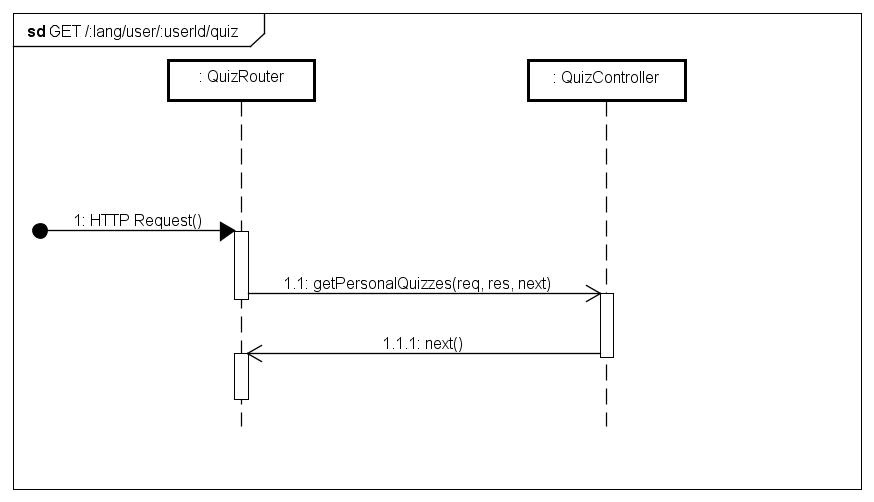
\includegraphics[scale=0.55]{UML/DiagrammiDiSequenza/Back-end/GET__lang_user_userId_quiz_success.png}
	\caption{Procedura di visualizzazione questionari creati}
\end{figure}
\FloatBarrier

\item \textbf{Fallimento}: questo scenario rappresenta il fallimento di una richiesta di visualizzazione dei questionari creati che impone, come vincolo per poter essere effettuata, che l'utente sia autenticato al sistema e sia un utente pro; quindi prima di tale operazione deve venire fatta una richiesta di controllo di sessione mediante l'apposita risorsa \textit{REST\ped{G}}. In questo caso il modulo \texttt{QuizController} invia \texttt{next(error)} per indicare il fallimento di tale vincolo al router il quale avrà compito di reinstradarlo (indirizzandolo verso \texttt{ErrorHandler}).
\label{Fallimento della procedura di visualizzazione questionari creati}
\begin{figure}[ht]
	\centering
	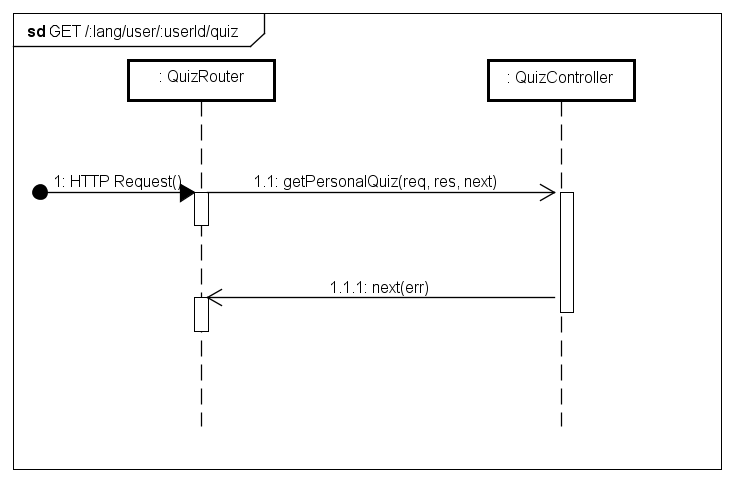
\includegraphics[scale=0.55]{UML/DiagrammiDiSequenza/Back-end/GET__lang_user_userId_quiz_failure.png}
	\caption{Fallimento della procedura di visualizzazione questionari creati}
\end{figure}
\FloatBarrier
\end{itemize}

\paragraph{GET /:lang/user/:userId/quiz/:quizId} % Restituisce il questionario creato dall'utente pro
\begin{itemize}
\item \textbf{Successo}: questo scenario rappresenta il successo di una richiesta di visualizzazione del questionario creato dall'utente che impone, come vincolo per poter essere effettuata, che l'utente sia autenticato come utente pro; quindi prima di tale operazione deve venire fatta una richiesta di controllo di sessione mediante l'apposita risorsa \textit{REST\ped{G}}. In questo caso il modulo \texttt{QuizController} invia \texttt{next()} per indicare il successo dell'operazione.
\label{Procedura di visualizzazione questionario creato}
\begin{figure}[ht]
	\centering
	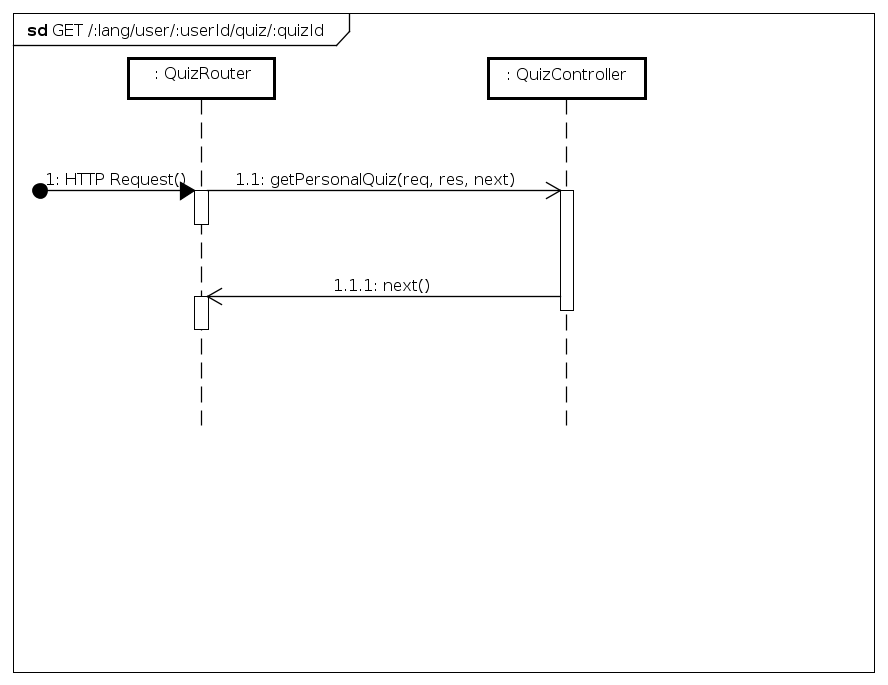
\includegraphics[scale=0.40]{UML/DiagrammiDiSequenza/Back-end/GET__lang_user_userId_quiz_quizId_success.png}
	\caption{Procedura di visualizzazione questionari creati}
\end{figure}
\FloatBarrier

\item \textbf{Fallimento}: questo scenario rappresenta il fallimento di una richiesta di visualizzazione del questionario creato che impone, come vincolo per poter essere effettuata, che l'utente sia autenticato al sistema e sia un utente pro; quindi prima di tale operazione deve venire fatta una richiesta di controllo di sessione mediante l'apposita risorsa \textit{REST\ped{G}}. In questo caso il modulo \texttt{QuizController} invia \texttt{next(error)} per indicare il fallimento di tale vincolo al router il quale avrà compito di reinstradarlo (indirizzandolo verso \texttt{ErrorHandler}).
\label{Fallimento della procedura di visualizzazione questionario creato}
\begin{figure}[ht]
	\centering
	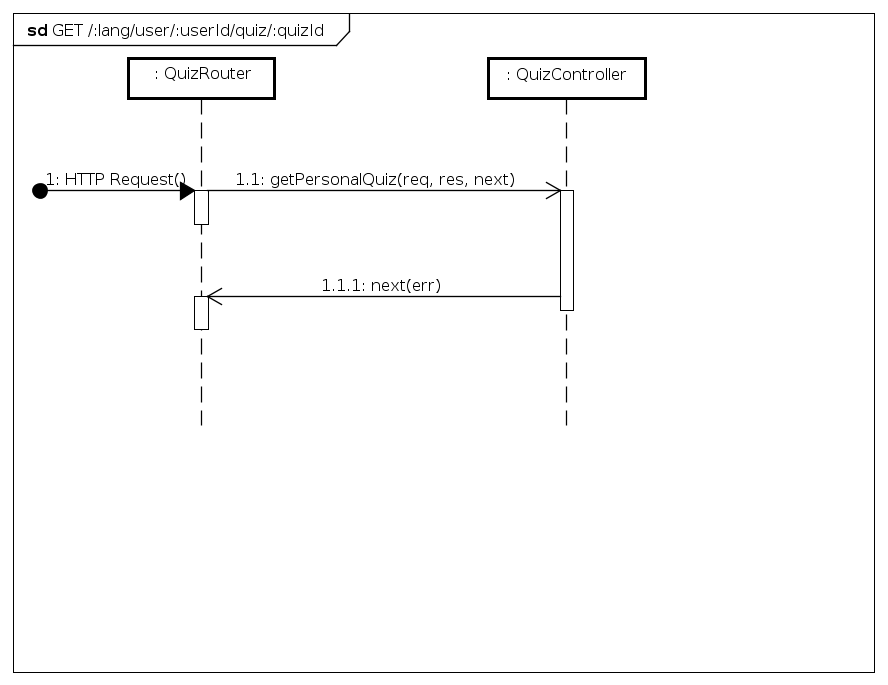
\includegraphics[scale=0.40]{UML/DiagrammiDiSequenza/Back-end/GET__lang_user_userId_quiz_quizId_failure.png}
	\caption{Fallimento della procedura di visualizzazione questionari creati}
\end{figure}
\FloatBarrier
\end{itemize}



\paragraph{POST /:lang/user/:useId/quiz} % Aggiunge un questionario nel sistema, restituisce un messaggio di conferma o di errore
\begin{itemize}
\item \textbf{Successo}: questo scenario rappresenta il successo di una richiesta di creazione di un questionario che impone, come vincolo per poter essere effettuata, che l'utente sia autenticato al sistema e sia un utente pro; quindi prima di tale operazione deve venire fatta una richiesta di controllo di sessione mediante l'apposita risorsa \textit{REST\ped{G}}. In questo caso il modulo \texttt{QuizController} invia \texttt{next()} per indicare il successo dell'operazione.
\label{Procedura di creazione di un questionario}
\begin{figure}[ht]
	\centering
	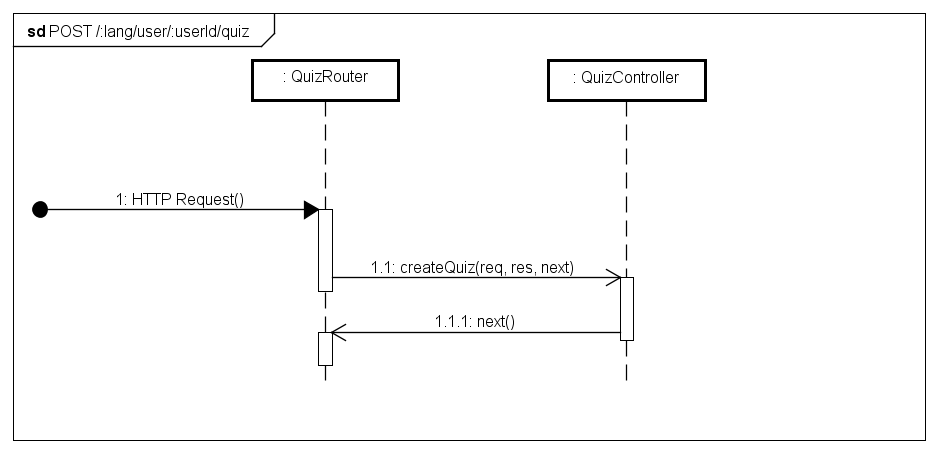
\includegraphics[scale=0.55]{UML/DiagrammiDiSequenza/Back-end/POST__lang_user_userId_quiz_success.png}
	\caption{Procedura di creazione di un questionario}
\end{figure}
\FloatBarrier

\item \textbf{Fallimento}: questo scenario rappresenta il fallimento di una richiesta di creazione di un questionario che impone, come vincolo per poter essere effettuata, che l'utente sia autenticato al sistema e sia un utente pro; quindi prima di tale operazione deve venire fatta una richiesta di controllo di sessione mediante l'apposita risorsa \textit{REST\ped{G}}. In questo caso il modulo \texttt{QuizController} invia \texttt{next(error)} per indicare il fallimento di tale vincolo al router il quale avrà compito di reinstradarlo (indirizzandolo verso \texttt{ErrorHandler}).
\label{Fallimento della procedura di creazione di un questionario}
\begin{figure}[ht]
	\centering
	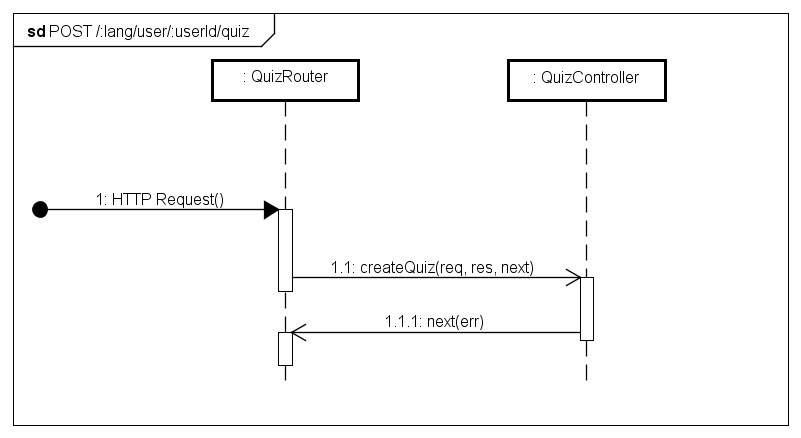
\includegraphics[scale=0.55]{UML/DiagrammiDiSequenza/Back-end/POST__lang_user_userId_quiz_failure.png}
	\caption{Fallimento della procedura di creazione di un questionario}
\end{figure}
\FloatBarrier
\end{itemize}

\paragraph{PUT /:lang/user/:userId/quiz/:quizId/removeUser} % Rimuove gli utenti iscritti al questionario 
\begin{itemize}
\item \textbf{Successo}: questo scenario rappresenta il successo di una richiesta di eliminazione di utente iscritto ad un questionario creato dall'utente che impone, come vincolo per poter essere effettuata, che l'utente sia autenticato come utente pro; quindi prima di tale operazione deve venire fatta una richiesta di controllo di sessione mediante l'apposita risorsa \textit{REST\ped{G}}. In questo caso il modulo \texttt{QuizController} invia \texttt{next()} per indicare il successo dell'operazione.
\label{Procedura di rimozione di utente iscritto ad un questionario}
\begin{figure}[ht]
	\centering
	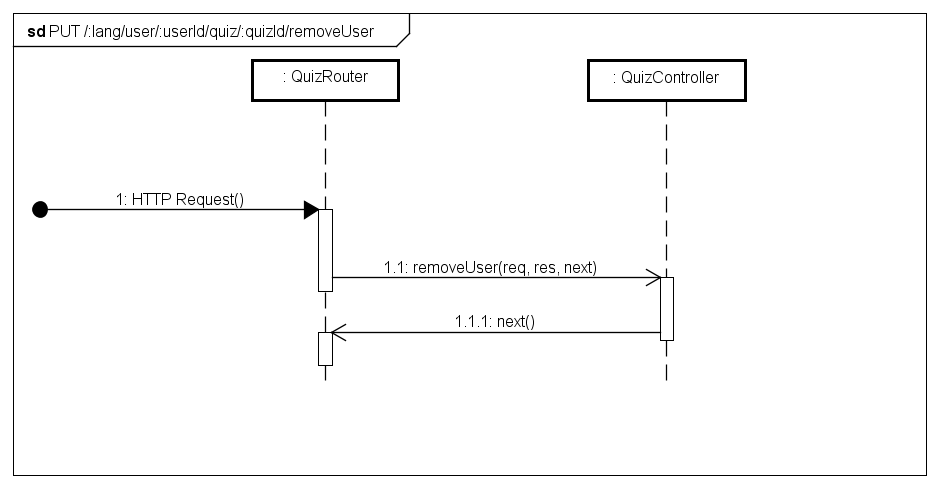
\includegraphics[scale=0.50]{UML/DiagrammiDiSequenza/Back-end/PUT_lang_user__userId_quiz__quizIdRemoveUserSuccess.png}
	\caption{Procedura di rimozione di un utente iscritto ad un questionario creato}
\end{figure}
\FloatBarrier

\item \textbf{Fallimento}: questo scenario rappresenta il fallimento di una richiesta di eliminazione di utente iscritto ad un questionario creato dall'utente che impone, come vincolo per poter essere effettuata, che l'utente sia autenticato al sistema e sia un utente pro; quindi prima di tale operazione deve venire fatta una richiesta di controllo di sessione mediante l'apposita risorsa \textit{REST\ped{G}}. In questo caso il modulo \texttt{QuizController} invia \texttt{next(error)} per indicare il fallimento di tale vincolo al router il quale avrà compito di reinstradarlo (indirizzandolo verso \texttt{ErrorHandler}).
\label{Fallimento della procedura di rimozione di un utente iscritto ad un questionario creato}
\begin{figure}[ht]
	\centering
	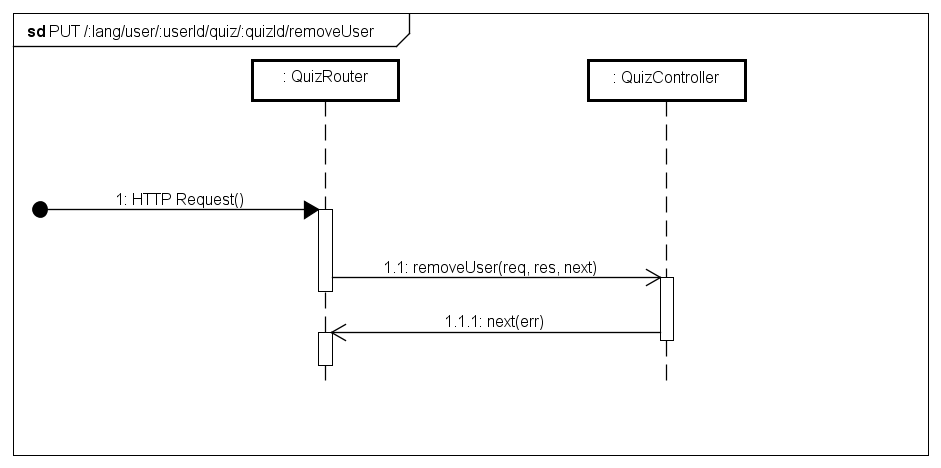
\includegraphics[scale=0.50]{UML/DiagrammiDiSequenza/Back-end/PUT_LangUserUserIdQuizQuizIdRemoveUserFailure.png}
	\caption{Fallimento della procedura di visualizzazione questionari creati}
\end{figure}
\FloatBarrier
\end{itemize}


\paragraph{POST /:lang/user/:userId/quiz/:quizId/addUser} % Iscrive un utente ad un questionario, restituisce un messaggio di conferma o di errore
\begin{itemize}
\item \textbf{Successo}: questo scenario rappresenta il successo di una richiesta di iscrizione ad un questionario che impone, come vincolo per poter essere effettuata, che l'utente sia autenticato al sistema; quindi prima di tale operazione deve venire fatta una richiesta di controllo di sessione mediante l'apposita risorsa \textit{REST\ped{G}}. In questo caso il modulo \texttt{QuizController} invia \texttt{next()} per indicare il successo dell'operazione.
\label{Procedura di iscrizione ad un questionario}
\begin{figure}[ht]
	\centering
	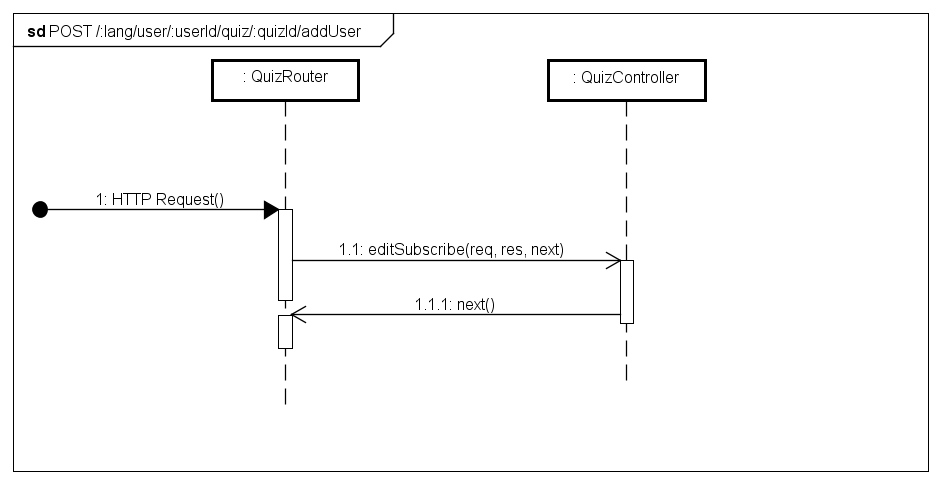
\includegraphics[scale=0.50]{UML/DiagrammiDiSequenza/Back-end/POST__lang_user_userId_quiz_quizId_addUser_success.png}
	\caption{Procedura di iscrizione ad un questionario}
\end{figure}
\FloatBarrier

\item \textbf{Fallimento}: questo scenario rappresenta il fallimento di una richiesta di iscrizione ad un questionario che impone, come vincolo per poter essere effettuata, che l'utente sia autenticato al sistema; quindi prima di tale operazione deve venire fatta una richiesta di controllo di sessione mediante l'apposita risorsa \textit{REST\ped{G}}. In questo caso il modulo \texttt{QuizController} invia \texttt{next(error)} per indicare il fallimento di tale vincolo al router il quale avrà compito di reinstradarlo (indirizzandolo verso \texttt{ErrorHandler}).
\label{Fallimento della procedura di iscrizione ad un questionario}
\begin{figure}[ht]
	\centering
	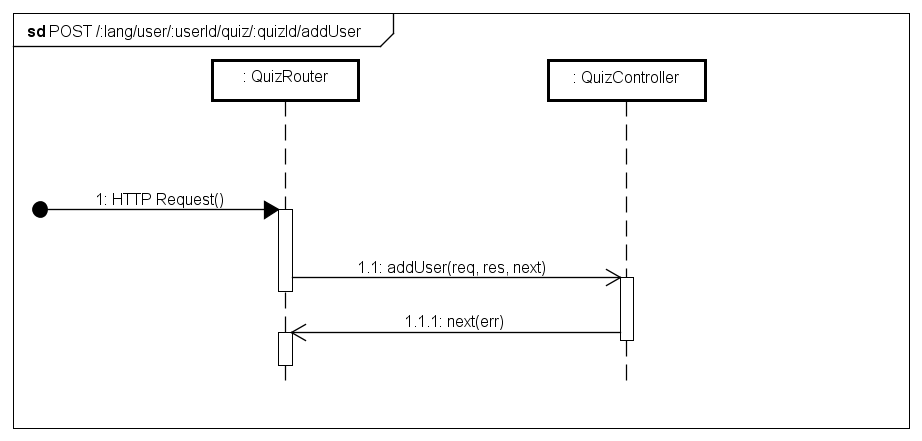
\includegraphics[scale=0.50]{UML/DiagrammiDiSequenza/Back-end/POST__lang_user_userId_quiz_quizId_addUser_failure.png}
	\caption{Fallimento della procedura di iscrizione ad un questionario}
\end{figure}
\FloatBarrier
\end{itemize}

\paragraph{POST /:lang/user/:userId/quiz/:quizId/activeUser} % Aggiunge un utente iscritto al questionario nella lista degli utenti che lo hanno eseguito
\begin{itemize}
\item \textbf{Successo}: questo scenario rappresenta il successo di una richiesta di aggiunta alla lista di utenti che hanno compilato un questionario che impone, come vincolo per poter essere effettuata, che l'utente sia autenticato al sistema; quindi prima di tale operazione deve venire fatta una richiesta di controllo di sessione mediante l'apposita risorsa \textit{REST\ped{G}}. In questo caso il modulo \texttt{QuizController} invia \texttt{next()} per indicare il successo dell'operazione.
\label{Procedura di aggiunta alla lista di utenti che hanno compilato un questionario}
\begin{figure}[ht]
	\centering
	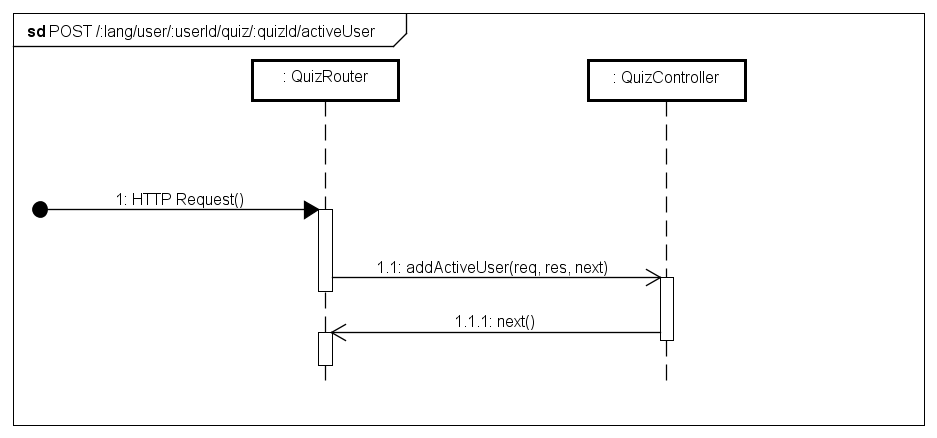
\includegraphics[scale=0.50]{UML/DiagrammiDiSequenza/Back-end/POST__lang_user_userId_quiz_quizId_activeUser_success.png}
	\caption{Procedura di aggiunta alla lista di utenti che hanno compilato un questionario}
\end{figure}
\FloatBarrier

\item \textbf{Fallimento}: questo scenario rappresenta il fallimento di una richiesta di aggiunta alla lista di utenti che hanno compilato un questionario che impone, come vincolo per poter essere effettuata, che l'utente sia autenticato al sistema; quindi prima di tale operazione deve venire fatta una richiesta di controllo di sessione mediante l'apposita risorsa \textit{REST\ped{G}}. In questo caso il modulo \texttt{QuizController} invia \texttt{next(error)} per indicare il fallimento di tale vincolo al router il quale avrà compito di reinstradarlo (indirizzandolo verso \texttt{ErrorHandler}).
\label{Fallimento della procedura di aggiunta alla lista di utenti che hanno compilato un questionario}
\begin{figure}[ht]
	\centering
	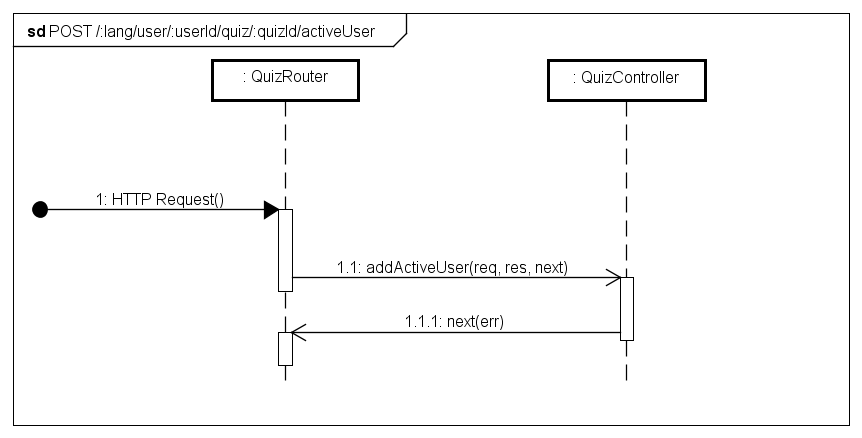
\includegraphics[scale=0.40]{UML/DiagrammiDiSequenza/Back-end/POST__lang_user_userId_quiz_quizId_activeUser_failure.png}
	\caption{Fallimento della procedura di aggiunta alla lista di utenti che hanno compilato un questionario}
\end{figure}
\FloatBarrier
\end{itemize}

\paragraph{PUT /:lang/user/:userId/quiz/:quizId} % Modifica di un questionario creato in precedenza, restituisce un messaggio di conferma o di errore
\begin{itemize}
\item \textbf{Successo}: questo scenario rappresenta il successo di una richiesta di modifica di un questionario che impone, come vincolo per poter essere effettuata, che l'utente sia autenticato al sistema e sia l'utente pro che aveva creato il questionario che si vuole modificare; quindi prima di tale operazione deve venire fatta una richiesta di controllo di sessione mediante l'apposita risorsa \textit{REST\ped{G}}. In questo caso il modulo \texttt{QuizController} invia \texttt{next()} per indicare il successo dell'operazione.
\label{Procedura di modifica di un questionario}
\begin{figure}[ht]
	\centering
	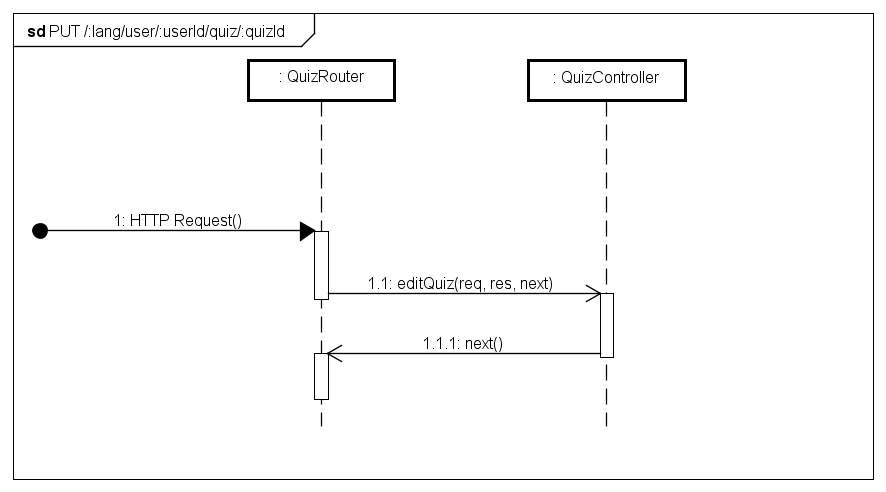
\includegraphics[scale=0.50]{UML/DiagrammiDiSequenza/Back-end/PUT__lang_user_userId_quiz_quizId_success.png}
	\caption{Procedura di modifica di un questionario}
\end{figure}
\FloatBarrier

\item \textbf{Fallimento}: questo scenario rappresenta il fallimento di una richiesta di modifica di un questionario che impone, come vincolo per poter essere effettuata, che l'utente sia autenticato al sistema e sia l'utente pro che aveva creato il questionario che si vuole modificare; quindi prima di tale operazione deve venire fatta una richiesta di controllo di sessione mediante l'apposita risorsa \textit{REST\ped{G}}. In questo caso il modulo \texttt{QuizController} invia \texttt{next(error)} per indicare il fallimento di tale vincolo al router il quale avrà compito di reinstradarlo (indirizzandolo verso \texttt{ErrorHandler}).
\label{Fallimento della procedura di modifica di un questionario}
\begin{figure}[ht]
	\centering
	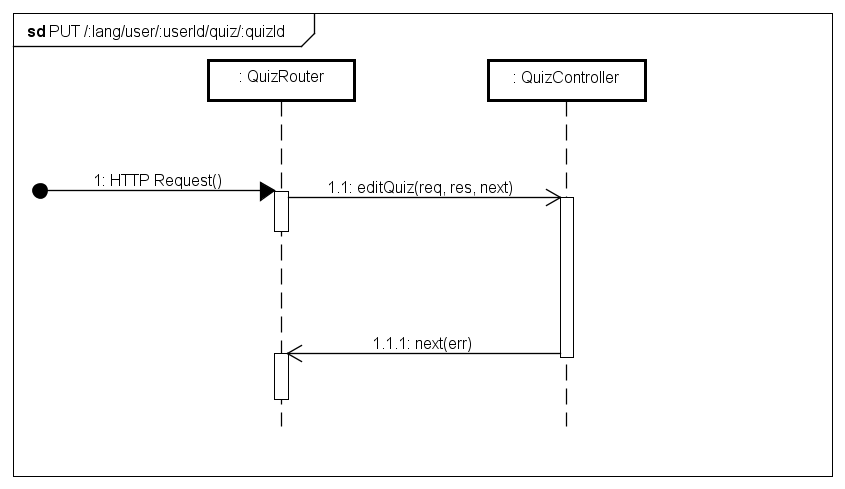
\includegraphics[scale=0.40]{UML/DiagrammiDiSequenza/Back-end/PUT__lang_user_userId_quiz_quizId_failure.png}
	\caption{Fallimento della procedura di modifica di un questionario}
\end{figure}
\FloatBarrier
\end{itemize}

\paragraph{GET /:lang/user/:userId/quiz/:quizId/test} % Restituisce il quiz selezionato dall'utente per effettuare l'esercitazione
\begin{itemize}
\item \textbf{Successo}: questo scenario rappresenta il successo di una richiesta di visualizzazione del questionario da compilare che impone, come vincolo per poter essere effettuata, che l'utente sia autenticato al sistema e che sia iscritto e in seguito abilitato a compilare il questionario; quindi prima di tale operazione deve venire fatta una richiesta di controllo di sessione mediante l'apposita risorsa \textit{REST\ped{G}}. In questo caso il modulo \texttt{QuizController} invia \texttt{next()} per indicare il successo dell'operazione.
\label{Procedura di visualizzazione del questionario da compilare}
\begin{figure}[ht]
	\centering
	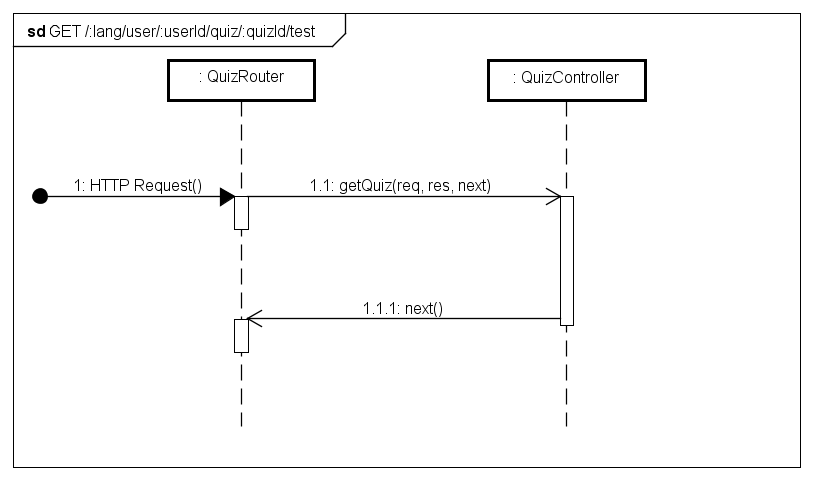
\includegraphics[scale=0.50]{UML/DiagrammiDiSequenza/Back-end/GET__lang_user_userId_quiz_quizId_test_success.png}
	\caption{Procedura di visualizzazione del questionario da compilare}
\end{figure}
\FloatBarrier

\item \textbf{Fallimento}: questo scenario rappresenta il fallimento di una richiesta di visualizzazione del questionario da compilare che impone, come vincolo per poter essere effettuata, che l'utente sia autenticato al sistema e che sia iscritto e in seguito abilitato a compilare il questionario; quindi prima di tale operazione deve venire fatta una richiesta di controllo di sessione mediante l'apposita risorsa \textit{REST\ped{G}}. In questo caso il modulo \texttt{QuizController} invia \texttt{next(error)} per indicare il fallimento di tale vincolo al router il quale avrà compito di reinstradarlo (indirizzandolo verso \texttt{ErrorHandler}).
\label{Fallimento della procedura di visualizzazione del questionario da compilare}
\begin{figure}[ht]
	\centering
	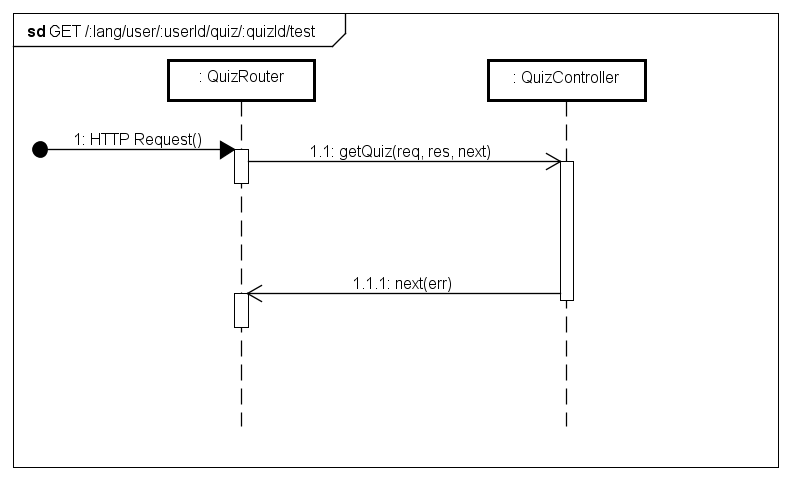
\includegraphics[scale=0.40]{UML/DiagrammiDiSequenza/Back-end/GET__lang_user_userId_quiz_quizId_test_failure.png}
	\caption{Fallimento della procedura di visualizzazione del questionario da compilare}
\end{figure}
\FloatBarrier
\end{itemize}

\paragraph{POST /:lang/user/:userId/quiz/:quizId/summary} % Crea il riepilogo del questionario svolto;
\begin{itemize}
\item \textbf{Successo}: questo scenario rappresenta il successo di una richiesta di creazione di un riepilogo che impone, come vincolo per poter essere effettuata, che l'utente sia autenticato al sistema e che abbia finito di compilare un questionario; quindi prima di tale operazione deve venire fatta una richiesta di controllo di sessione mediante l'apposita risorsa \textit{REST\ped{G}}. In questo caso il modulo \texttt{SummaryController} invia \texttt{next()} per indicare il successo dell'operazione e successivamente verrà effettuata la \texttt{updateSummary()} per aggiornare la cronologia dell'utente.
\label{Procedura di creazione di un riepilogo}
\begin{figure}[ht]
	\centering
	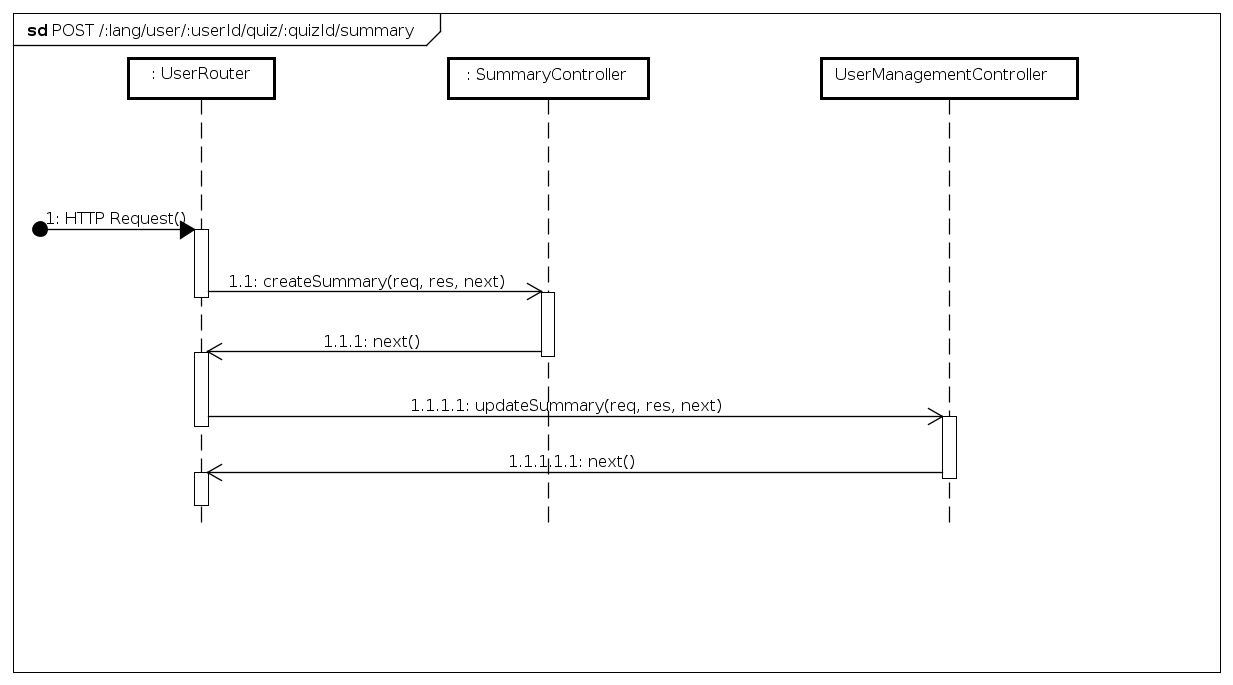
\includegraphics[scale=0.40]{UML/DiagrammiDiSequenza/Back-end/POST__lang_user_userId_quiz_quizId_summary_success.png}
	\caption{Procedura di creazione di un riepilogo}
\end{figure}
\FloatBarrier

\item \textbf{Fallimento}: questo scenario rappresenta il fallimento di una richiesta di creazione di un riepilogo che impone, come vincolo per poter essere effettuata, che l'utente sia autenticato al sistema e che abbia finito di compilare un questionario; quindi prima di tale operazione deve venire fatta una richiesta di controllo di sessione mediante l'apposita risorsa \textit{REST\ped{G}}. In questo caso il modulo \texttt{SummaryController} invia \texttt{next(error)} per indicare il fallimento di tale vincolo al router il quale avrà compito di reinstradarlo (indirizzandolo verso \texttt{ErrorHandler}).
\label{Fallimento della procedura di creazione di un riepilogo}
\begin{figure}[ht]
	\centering
	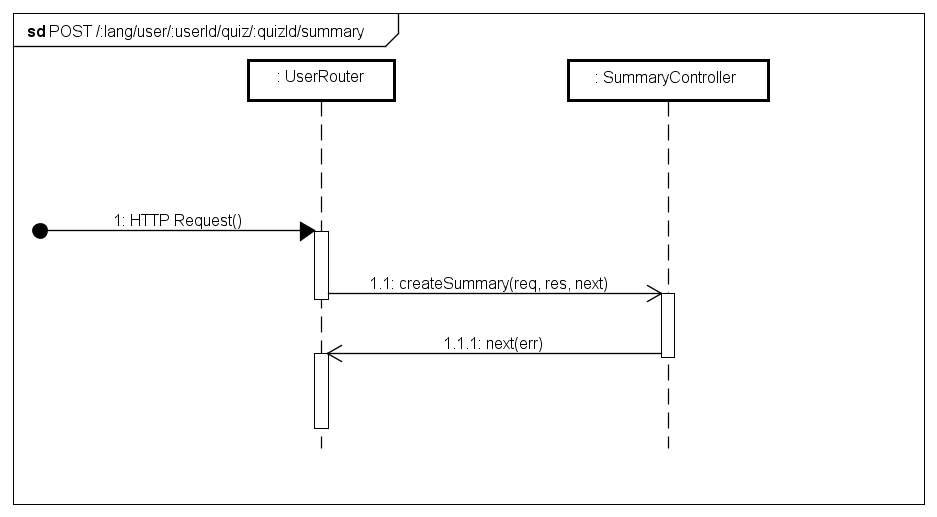
\includegraphics[scale=0.40]{UML/DiagrammiDiSequenza/Back-end/POST__lang_user_userId_quiz_quizId_summary_failure.png}
	\caption{Fallimento della procedura di creazione di un riepilogo}
\end{figure}
\FloatBarrier
\end{itemize}

